\documentclass{article}

\usepackage{tikz}
\usetikzlibrary{circuits.ee.IEC}

%\tikzset{circuit declare symbol=terminal}
%\tikzset{set terminal graphic={draw, generic circle IEC, minimum size=4pt}}
\tikzset{circuit declare symbol=voltmeter}
\tikzset{set voltmeter graphic={draw, generic circle IEC, minimum size=6mm, info=center:V}}

\begin{document}

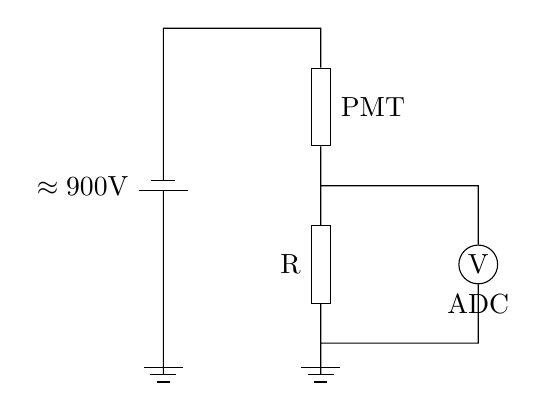
\begin{tikzpicture}[x=2cm,y=2cm,circuit ee IEC]
\draw (0, -.2) node[ground,point down] {} -- (0, 0) to[resistor={info=R}] (0, 1) -- (1, 1) to[voltmeter={info=right:ADC}] (1, 0) -- (0, 0);

\draw (-1, -.2) node[ground,point down] {} -- (-1, 0) to[battery={volt={\approx 900}}] (-1, 2) -- (0, 2) to[resistor={info={PMT}}] (0, 1);
\end{tikzpicture}

\end{document}